\section{Testing configurations}\label{sec:testing-configurations}

This section presents several test scenarios that were devised to evaluate the implemented localization system. They aim to test the accuracy and robustness of the implementation under different environmental conditions and hardware configurations.


\subsection{Testing platforms}

The localization system was tested on laser sensor data retrieved from three different mobile robot platforms and executed on the same computer in order to allow a direct comparison of computation time. This computer was a Clevo P370EM3 laptop (with a Intel Core i7 3630QM CPU at 2.4GHz, 16 GB of RAM DDR3, NVidia GTX680M graphics card and a Samsung 840 Pro SSD) and it was running Ubuntu 12.04 along with \gls{ros} Hydro, \gls{pcl} 1.7 and Gazebo 1.9.

The sensor data was recorded into rosbags, and is publicly available at\footnote{\url{https://github.com/carlosmccosta/dynamic_robot_localization_tests}} along with all the detailed results, configurations and experiments videos, in order to allow future comparisons with other localization systems. The hardware specifications of the \glspl{lidar} used is presented in \Cref{tab:localization-system-evaluation_laser-hardware-specifications} and the laser points after downsampling and registration can be seen on the movement paths figures as green dots (inliers) and red dots (outliers).


\subsubsection{Jarvis platform}

The Jarvis platform is an autonomous ground vehicle equipped with a SICK NAV 350 laser for self-localization (mounted about 2 meters from the floor) and a SICK S3000 laser for collision avoidance (mounted about 0.20 meters from the floor). It uses a tricycle locomotion system with two back wheels and a steerable wheel at the front. In \Cref{fig:localization-system-evaluation_jarvis} the robot is performing a delivery task with the package on top of a moving support. The 3 \gls{dof} ground truth was provided by the SICK NAV350 system and relied on 6 laser reflectors (with 9 cm of diameter) to perform the pose estimations (it is certified for robot docking operations with precision up to 4 millimeters).


\subsubsection{Pioneer 3-DX platform}

The Pioneer 3-DX shown in \Cref{fig:localization-system-evaluation_pioneer} is a small lightweight robot equipped with a SICK LMS-200 laser (mounted about 48 cm from the floor) and a Kinect (mounted about 78 cm from the floor). It uses a two-wheel two-motor differential drive locomotion system and can reach a linear speed of 1.2 m/s and angular velocity of 300º/s. The 3 \gls{dof} ground truth was provided by 8 Raptor-E cameras \footnote{\url{http://www.motionanalysis.com/html/movement/raptore.html}} and according to \cite{Sturm2012} it had less than 1 cm in translation error and less than 0.5 degrees in rotation error.

\begin{figure}[H]
	\centering
	\begin{minipage}[hb]{0.24\textwidth}
		\centering
		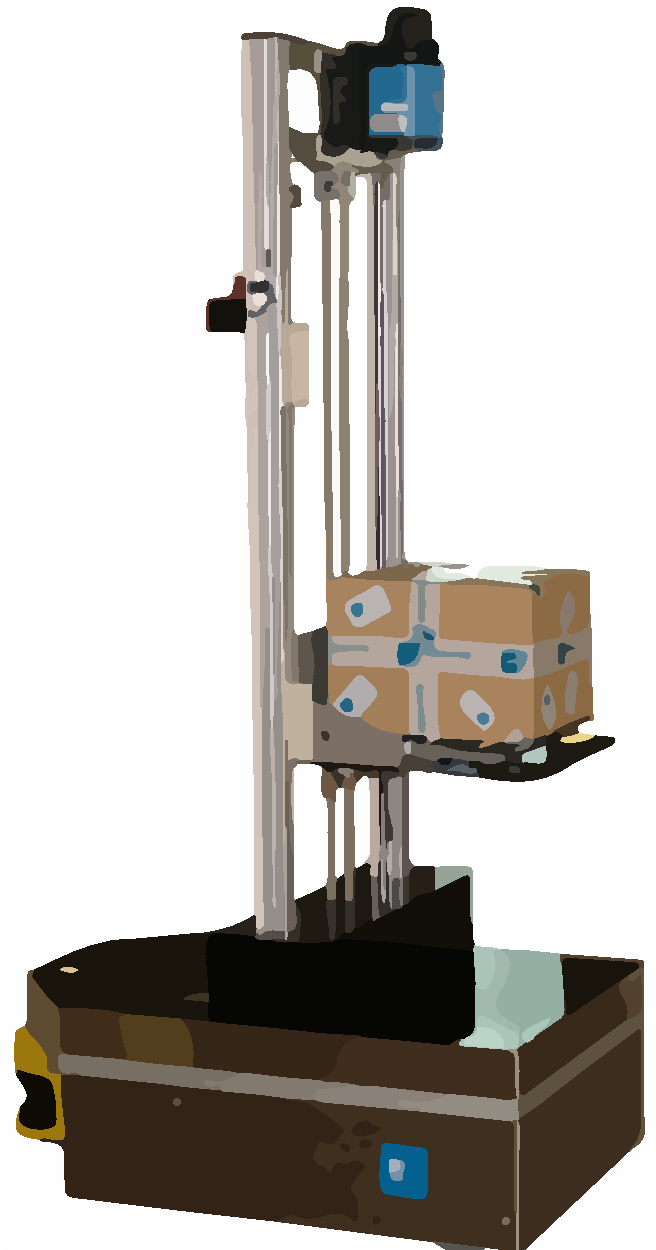
\includegraphics[width=0.8\textwidth]{localization-system-evaluation/testing-platforms/jarvis}
		\caption{Jarvis testing platform}
		\label{fig:localization-system-evaluation_jarvis}
	\end{minipage}\hfill
	\begin{minipage}[hb]{0.24\textwidth}
		\centering
		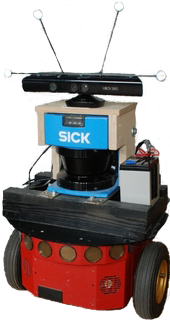
\includegraphics[width=0.7\textwidth]{localization-system-evaluation/testing-platforms/pioneer-3dx}
		\caption{Pioneer 3-DX testing platform \cite{Sturm2012}}
		\label{fig:localization-system-evaluation_pioneer}
	\end{minipage}
\end{figure}


\subsubsection{Guardian platform}

The Guardian platform is an autonomous mobile manipulator equipped with a Hokuyo URG-04LX laser in the front and a Hokuyo URG-04LX\_UG01 laser in the back (both mounted about 0.37 meters from the ground). The front laser had a tilting platform which allows 3D mapping of the environment. The arm is a SCHUNK Powerball LWA 4P and in \Cref{fig:localization-system-evaluation_guardian} it is attached to a stud welding machine (in simulation it is attached to a video projector). It uses a differential drive locomotion system and can be moved with wheels or with tracks. This platform didn't have a certified ground truth and as such, the results could not be quantified with an external localization system (the results performed with the Gazebo simulator will be presented instead - robot model shown in \Cref{fig:localization-system-evaluation_guardian_gazebo}).

\begin{figure}[H]
	\centering
	\begin{minipage}[hb]{0.24\textwidth}
		\centering
		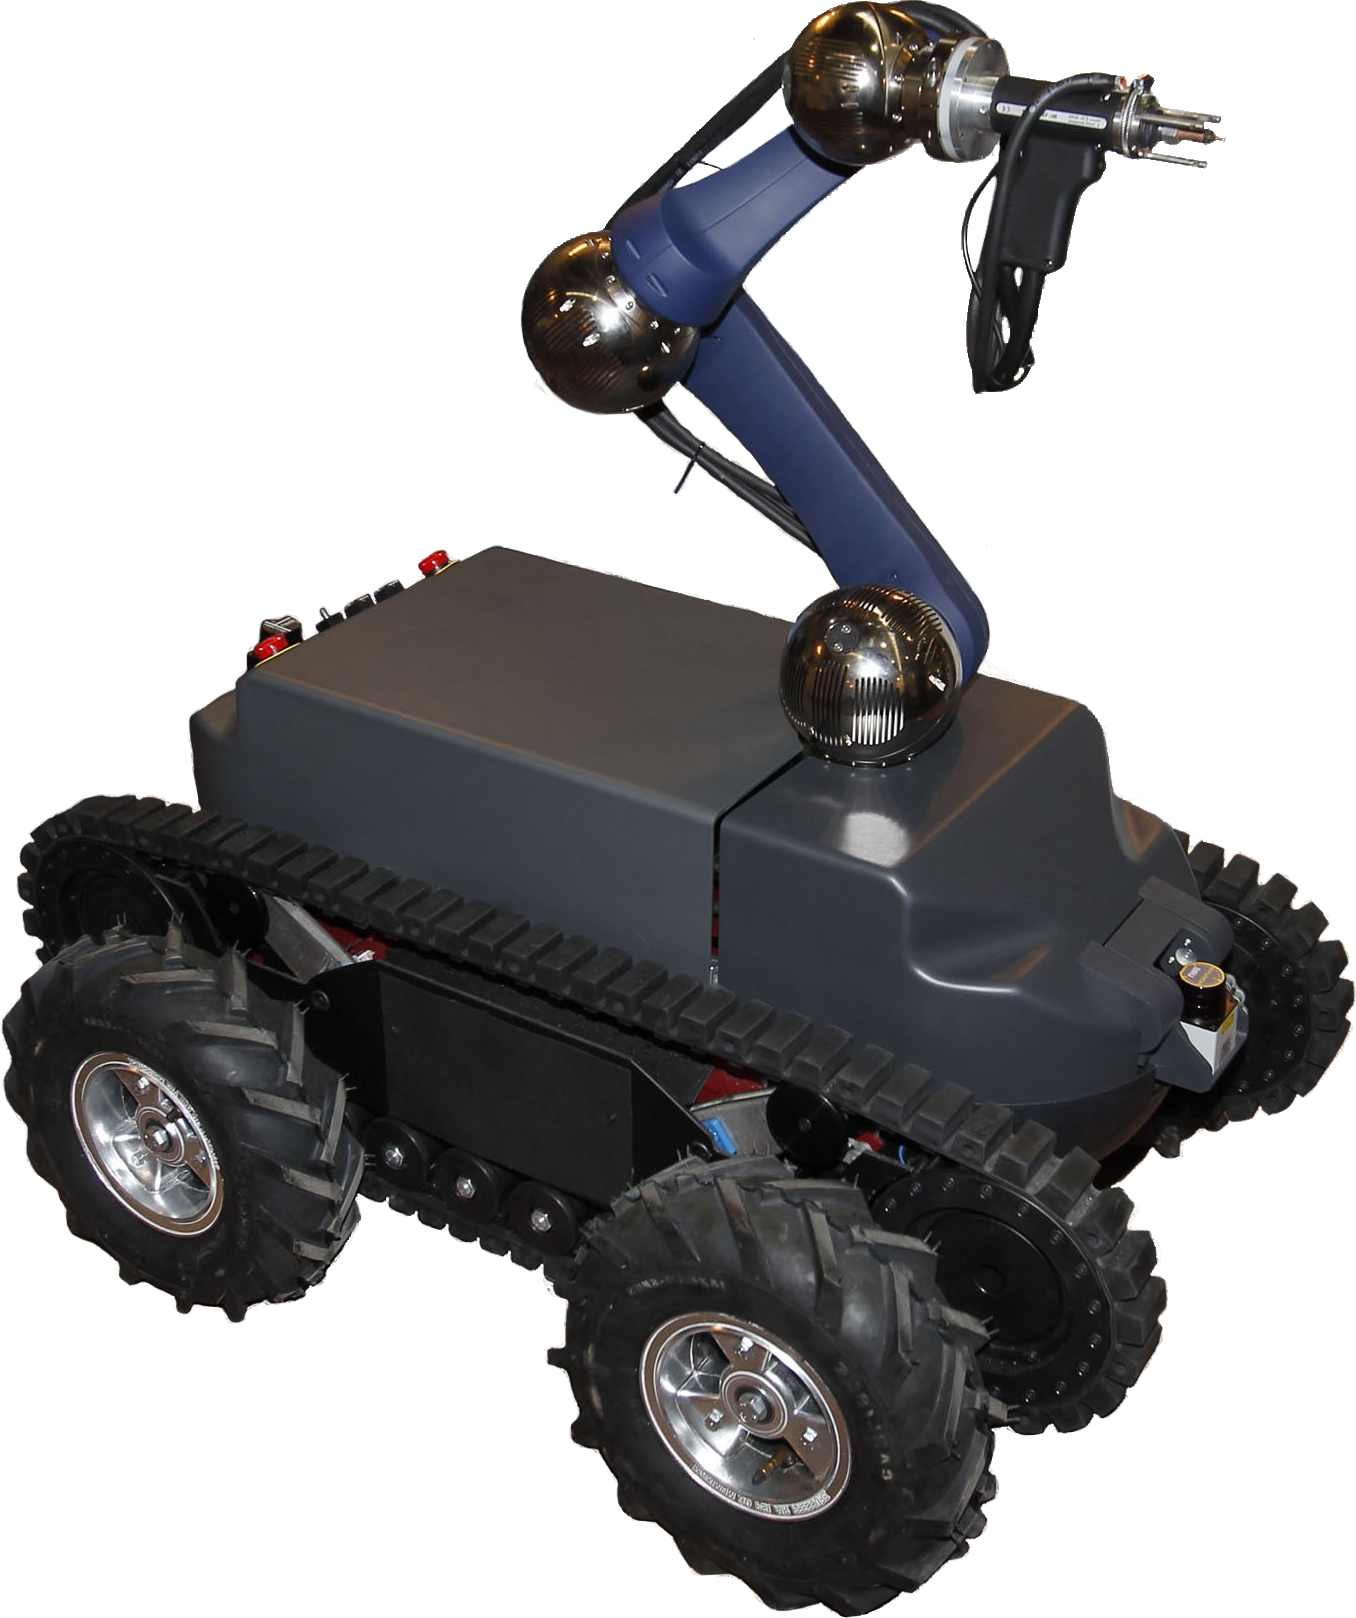
\includegraphics[width=0.84\textwidth]{localization-system-evaluation/testing-platforms/guardian}
		\caption{Guardian testing platform}
		\label{fig:localization-system-evaluation_guardian}
	\end{minipage}\hfill
	\begin{minipage}[hb]{0.24\textwidth}
		\centering
		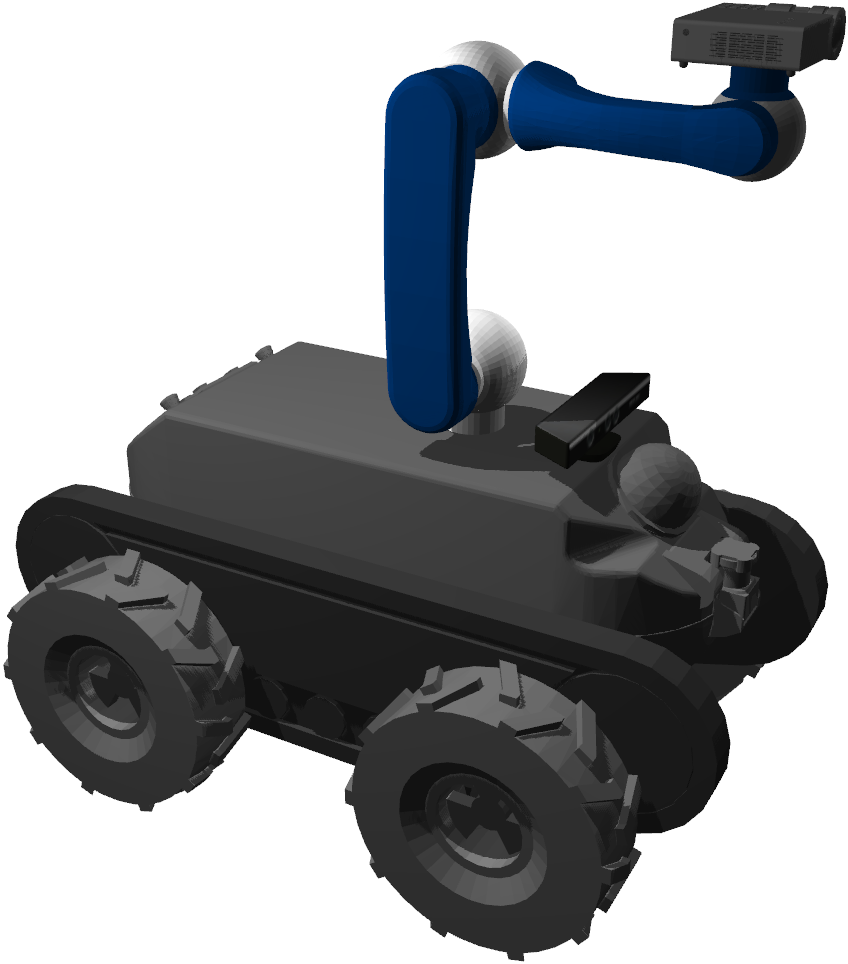
\includegraphics[width=0.84\textwidth]{localization-system-evaluation/testing-platforms/guardian-gazebo}
		\caption{Guardian Gazebo simulation}
		\label{fig:localization-system-evaluation_guardian_gazebo}
	\end{minipage}
\end{figure}


\begin{table*}[t]
	\caption{\glsentryplural{lidar} hardware specifications}
	\tabulinesep = 0.8ex
	\centering
	\small
	\begin{tabu} { X[2.5,m,c] | X[m,c] X[m,c] X[m,c] X[m,c] X[m,c] }
		\rowfont{\bfseries\itshape\small} Laser model & Range (meters) & Field of view (degrees) & Scanning frequency (Hz) & Angular resolution (degrees) & Statistical error (millimeters) \\
		\hline
		{\small SICK NAV350} 			& [0.5..250] 	& 360 	& 8 	& 0.25 	& 15 	\\
		{\small SICK S3000} 			& [0.1..49] 	& 190 	& 8 	& 0.25 	& 150 	\\
		{\small SICK LMS200} 			& [0.1..80] 	& 180 	& 10 	& 1.0 	& 35 	\\
		{\small Hokuyo URG-04LX} 		& [0.06..4.095] & 240 	& 10 	& 0.36 	& 10 	\\
		{\small Hokuyo URG-04LX\_UG01} 	& [0.02..4] 	& 240 	& 10 	& 0.36 	& 30 	\\
	\end{tabu}
	\label{tab:localization-system-evaluation_laser-hardware-specifications}
\end{table*}



\subsection{Testing environments}

The localization system was tested in different environments and used the Jarvis platform in a large room with a RoboCup field, the Pioneer 3-DX in a large industrial hall, the Guardian platform in a simulated indoor environment and a Kinect in a flying arena.


\subsubsection{Jarvis in RoboCup field}

The RoboCup field (shown in \Cref{fig:localization-system-evaluation_jarvis-tests-environment}) occupies half of a large room (with 20.5 meters of length and 7.7 meters of depth). It has two doors, several small windows and two large glass openings into the hallway. Several tests were performed with the robot at speeds ranging from 5 cm/s to 50 cm/s in this environment and up to 2 m/s using the Stage simulator\footnote{\url{http://rtv.github.io/Stage/}}. These tests were performed with two different movement paths. The first is a simple rounded path that aimed to test the robot in the region of space that had better ground truth (due to its position in relation to the laser reflectors). The second path was more complex and contained several sub paths with different velocities and shapes (it was intended to evaluate the localization system with typical movements that mobile manipulators require, such as moving forward and backwards with or without angular velocity and stopping at the desired destination).


\begin{figure}[H]
	\centering
	\begin{subfigure}[ht]{0.31\textwidth}
		\centering
		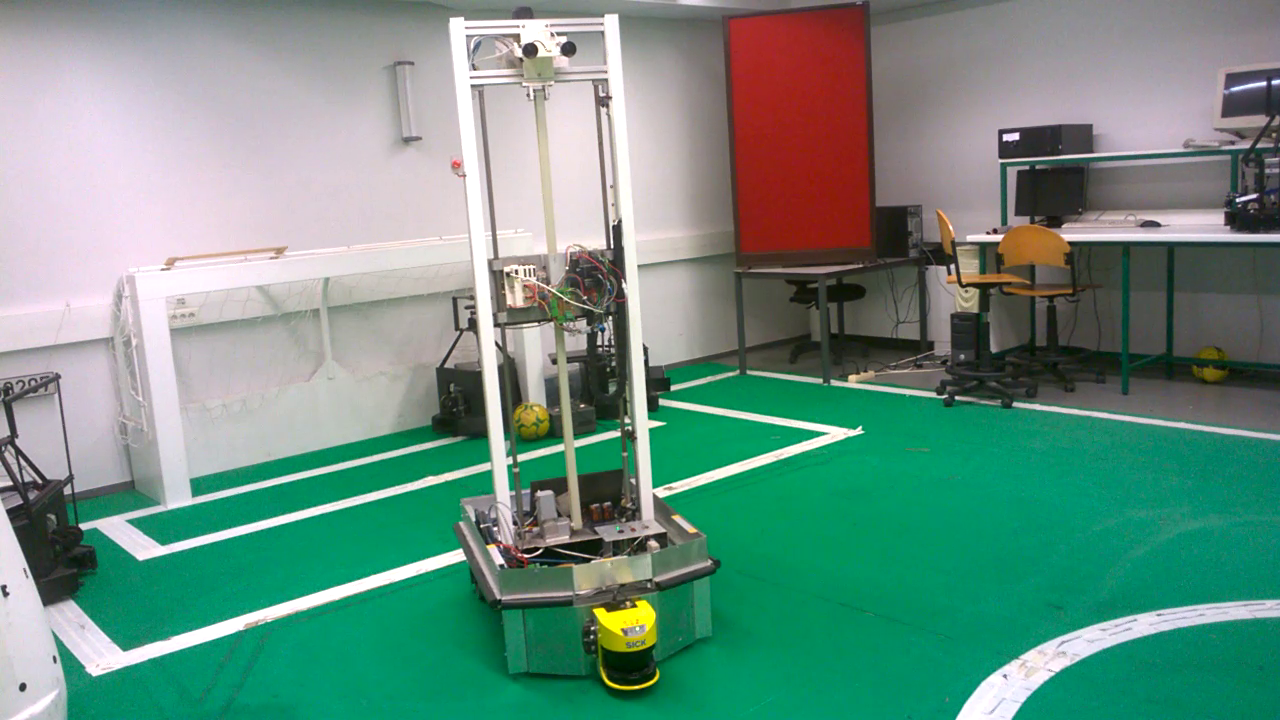
\includegraphics[width=\textwidth]{localization-system-evaluation/testing-environments/jarvis-environment-front-left}
	\end{subfigure}
	\begin{subfigure}[ht]{0.31\textwidth}
		\centering
		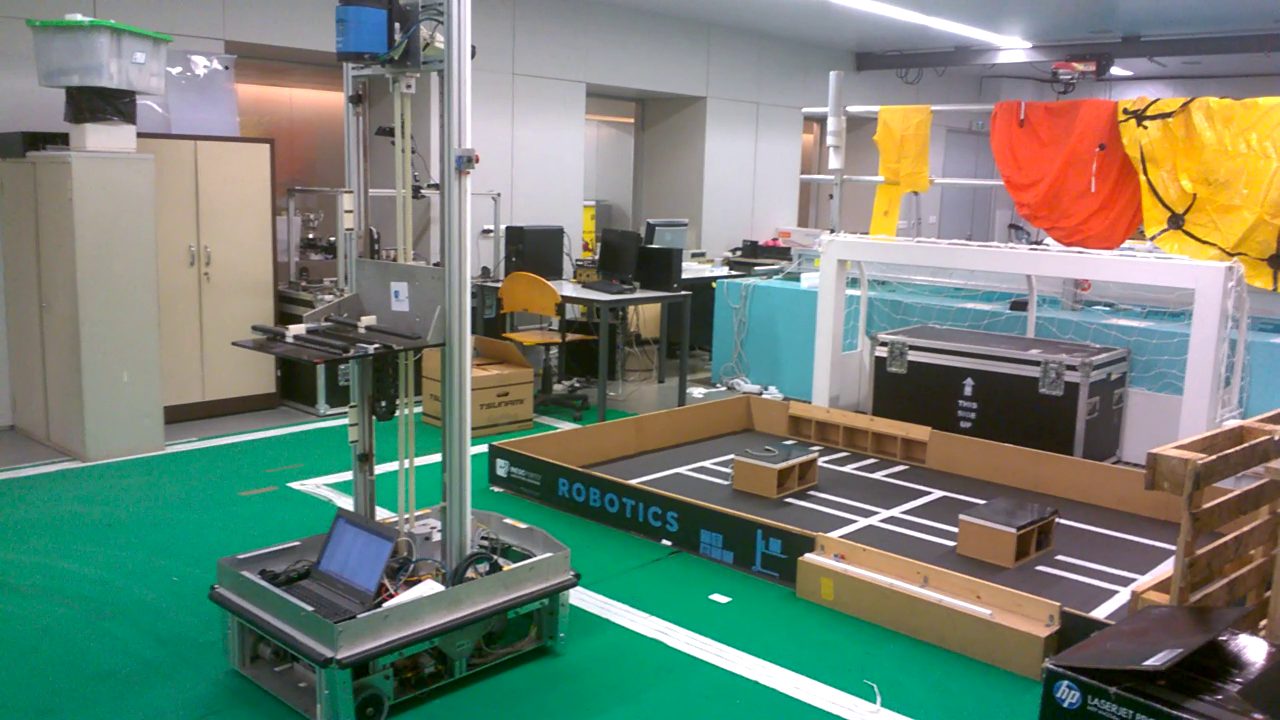
\includegraphics[width=\textwidth]{localization-system-evaluation/testing-environments/jarvis-environment-front-right}
	\end{subfigure}
	\caption{Jarvis testing environment}
	\label{fig:localization-system-evaluation_jarvis-tests-environment}
\end{figure}


\subsubsection{Guardian in structured environment}

The structured environment simulated in Gazebo is a large room with 12.4 meters of length and 8.4 meters of depth. It has 4 doors, several small windows and the walls have small ledges at regular intervals.

Given that the Guardian mobile manipulator is expected to work on the walls of this environment, several tests were devised with a path following the lower and right wall of the environment. The first test was done in a static environment clear of unknown objects and was meant to evaluate the best precision that the localization system could achieve. The second test was done in a cluttered environment and was designed to test the robustness of the localization system against static unknown objects, that were placed in the middle of the environment and close to the walls (to block sensor data from reaching known positions and analyze the robustness of matching unknown points that are close to known areas). The last test added a moving car to the scene and aimed to assess the impact of dynamic objects on the point cloud registration algorithms.


\begin{figure}[H]
	\centering
	\begin{subfigure}[ht]{0.25\textwidth}
		\centering
		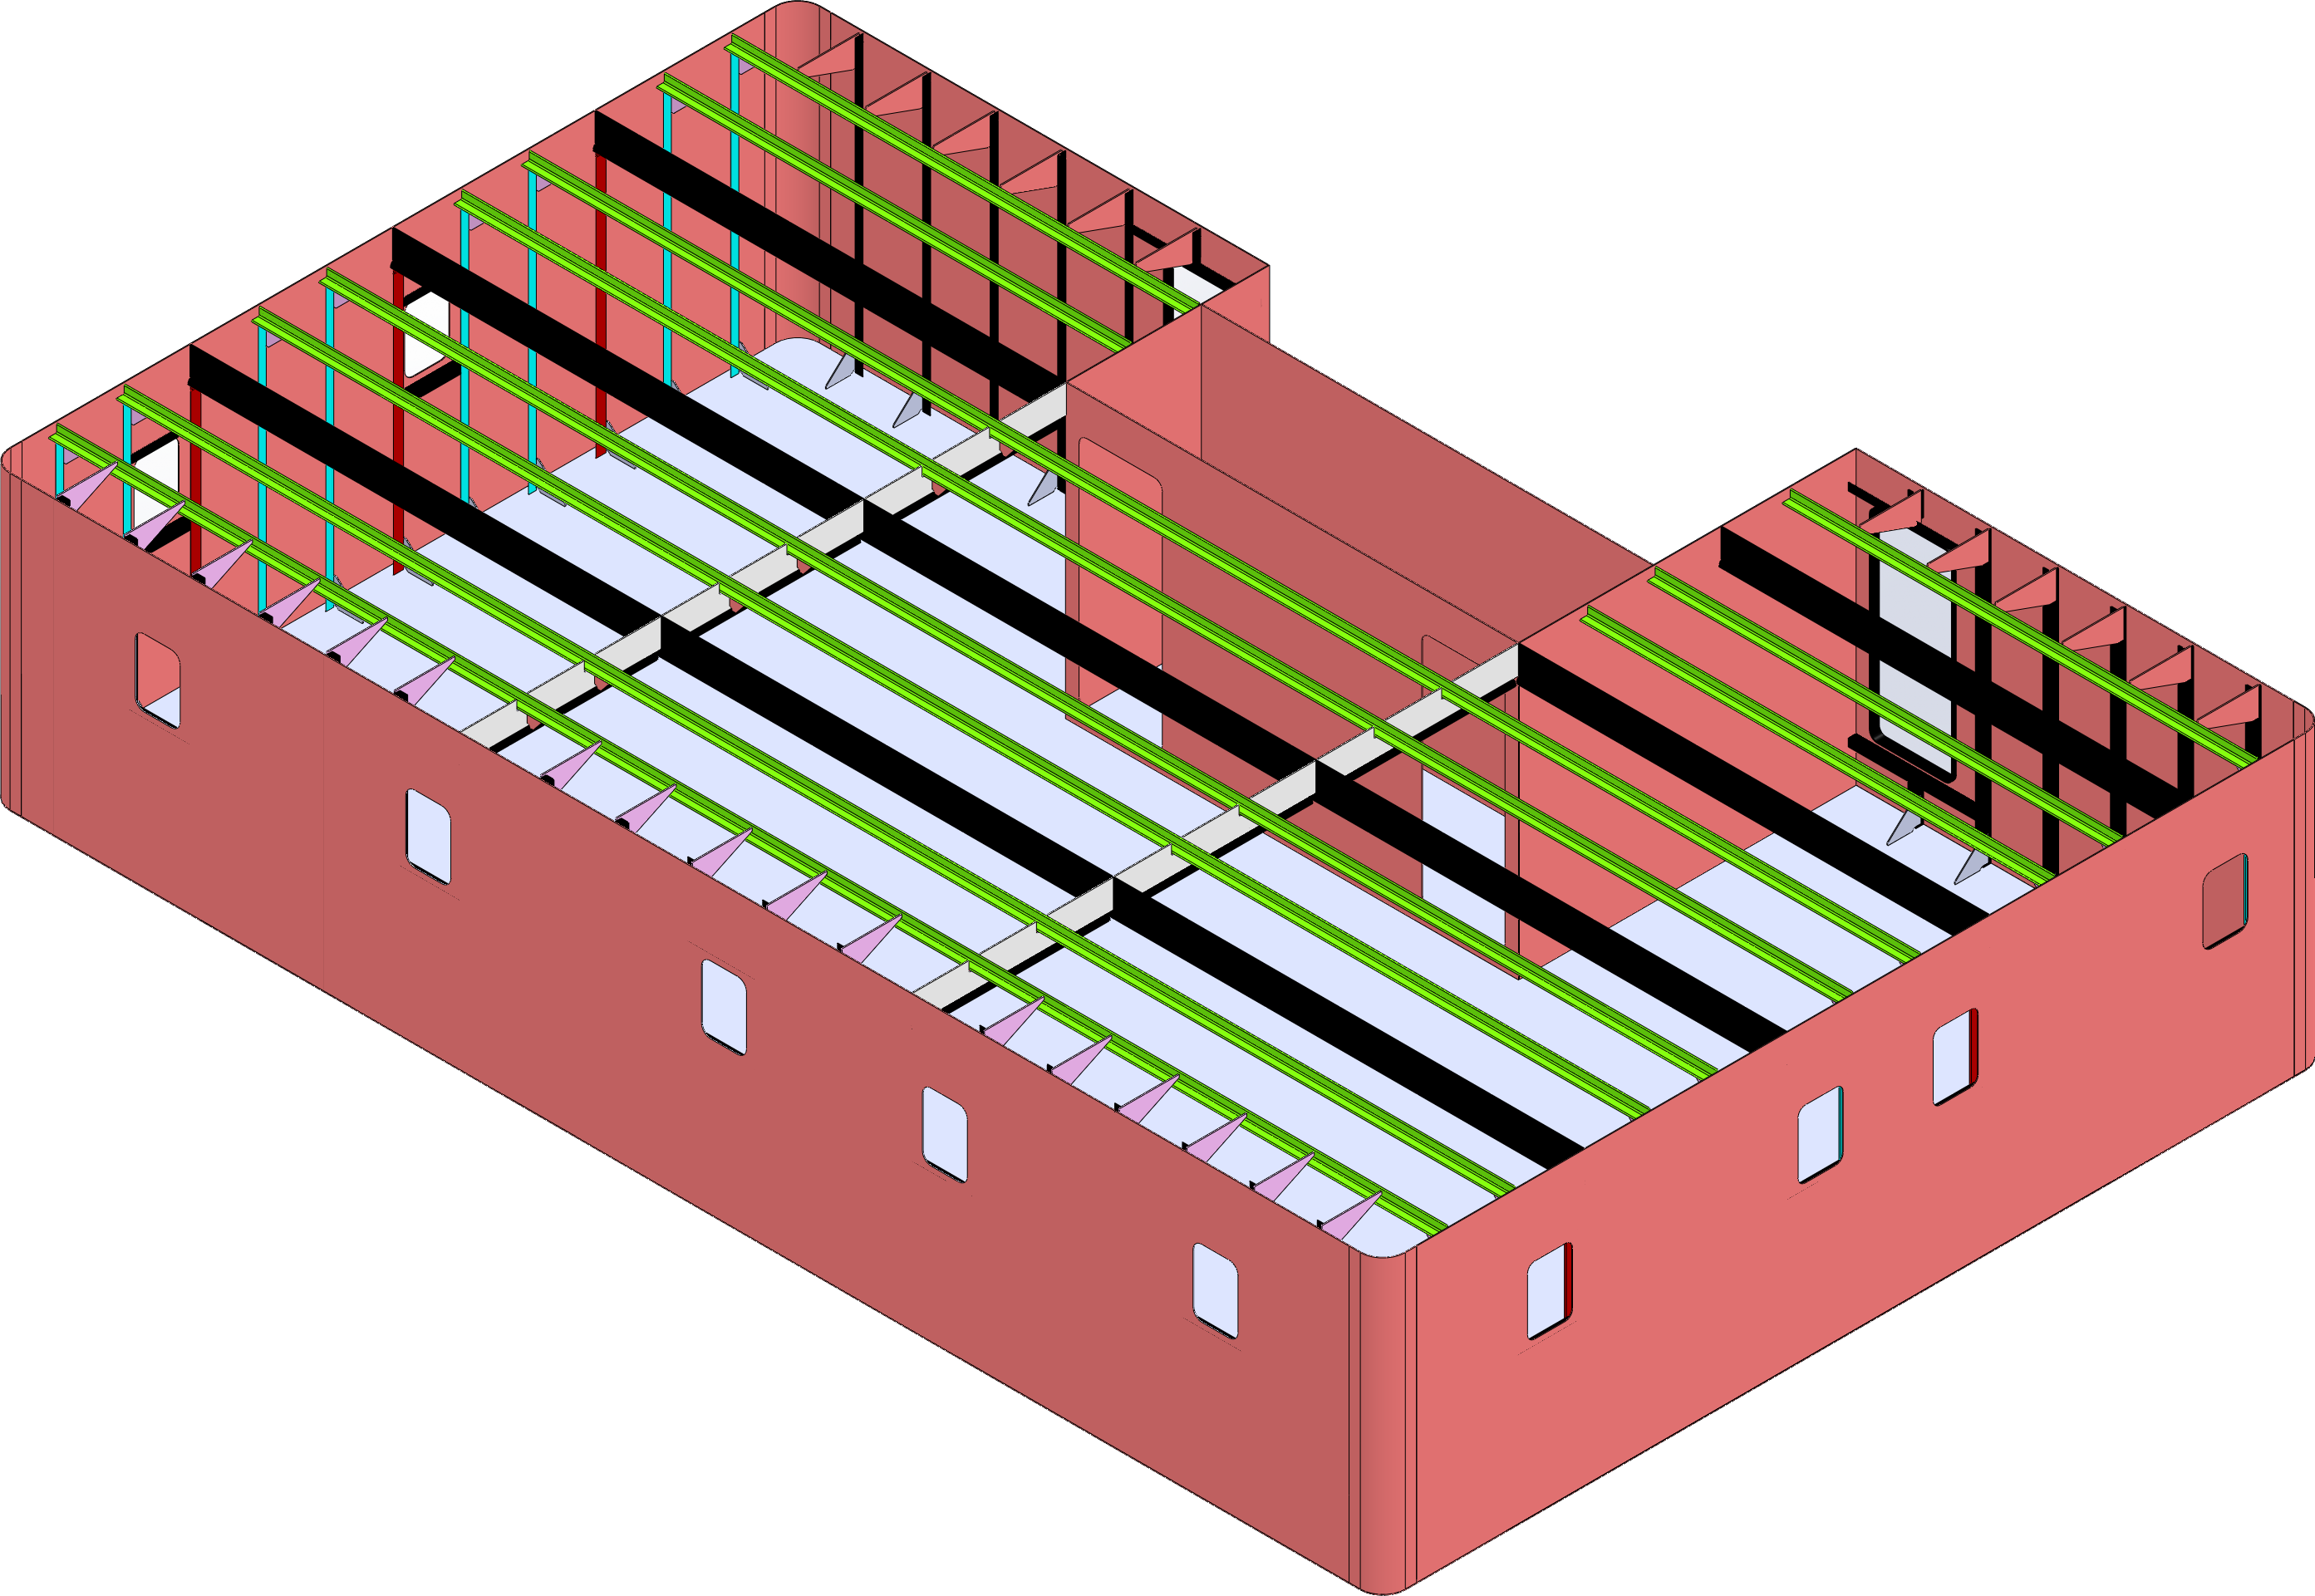
\includegraphics[width=\textwidth]{localization-system-evaluation/testing-environments/guardian-environment-corner}
	\end{subfigure}
	\begin{subfigure}[ht]{0.25\textwidth}
		\centering
		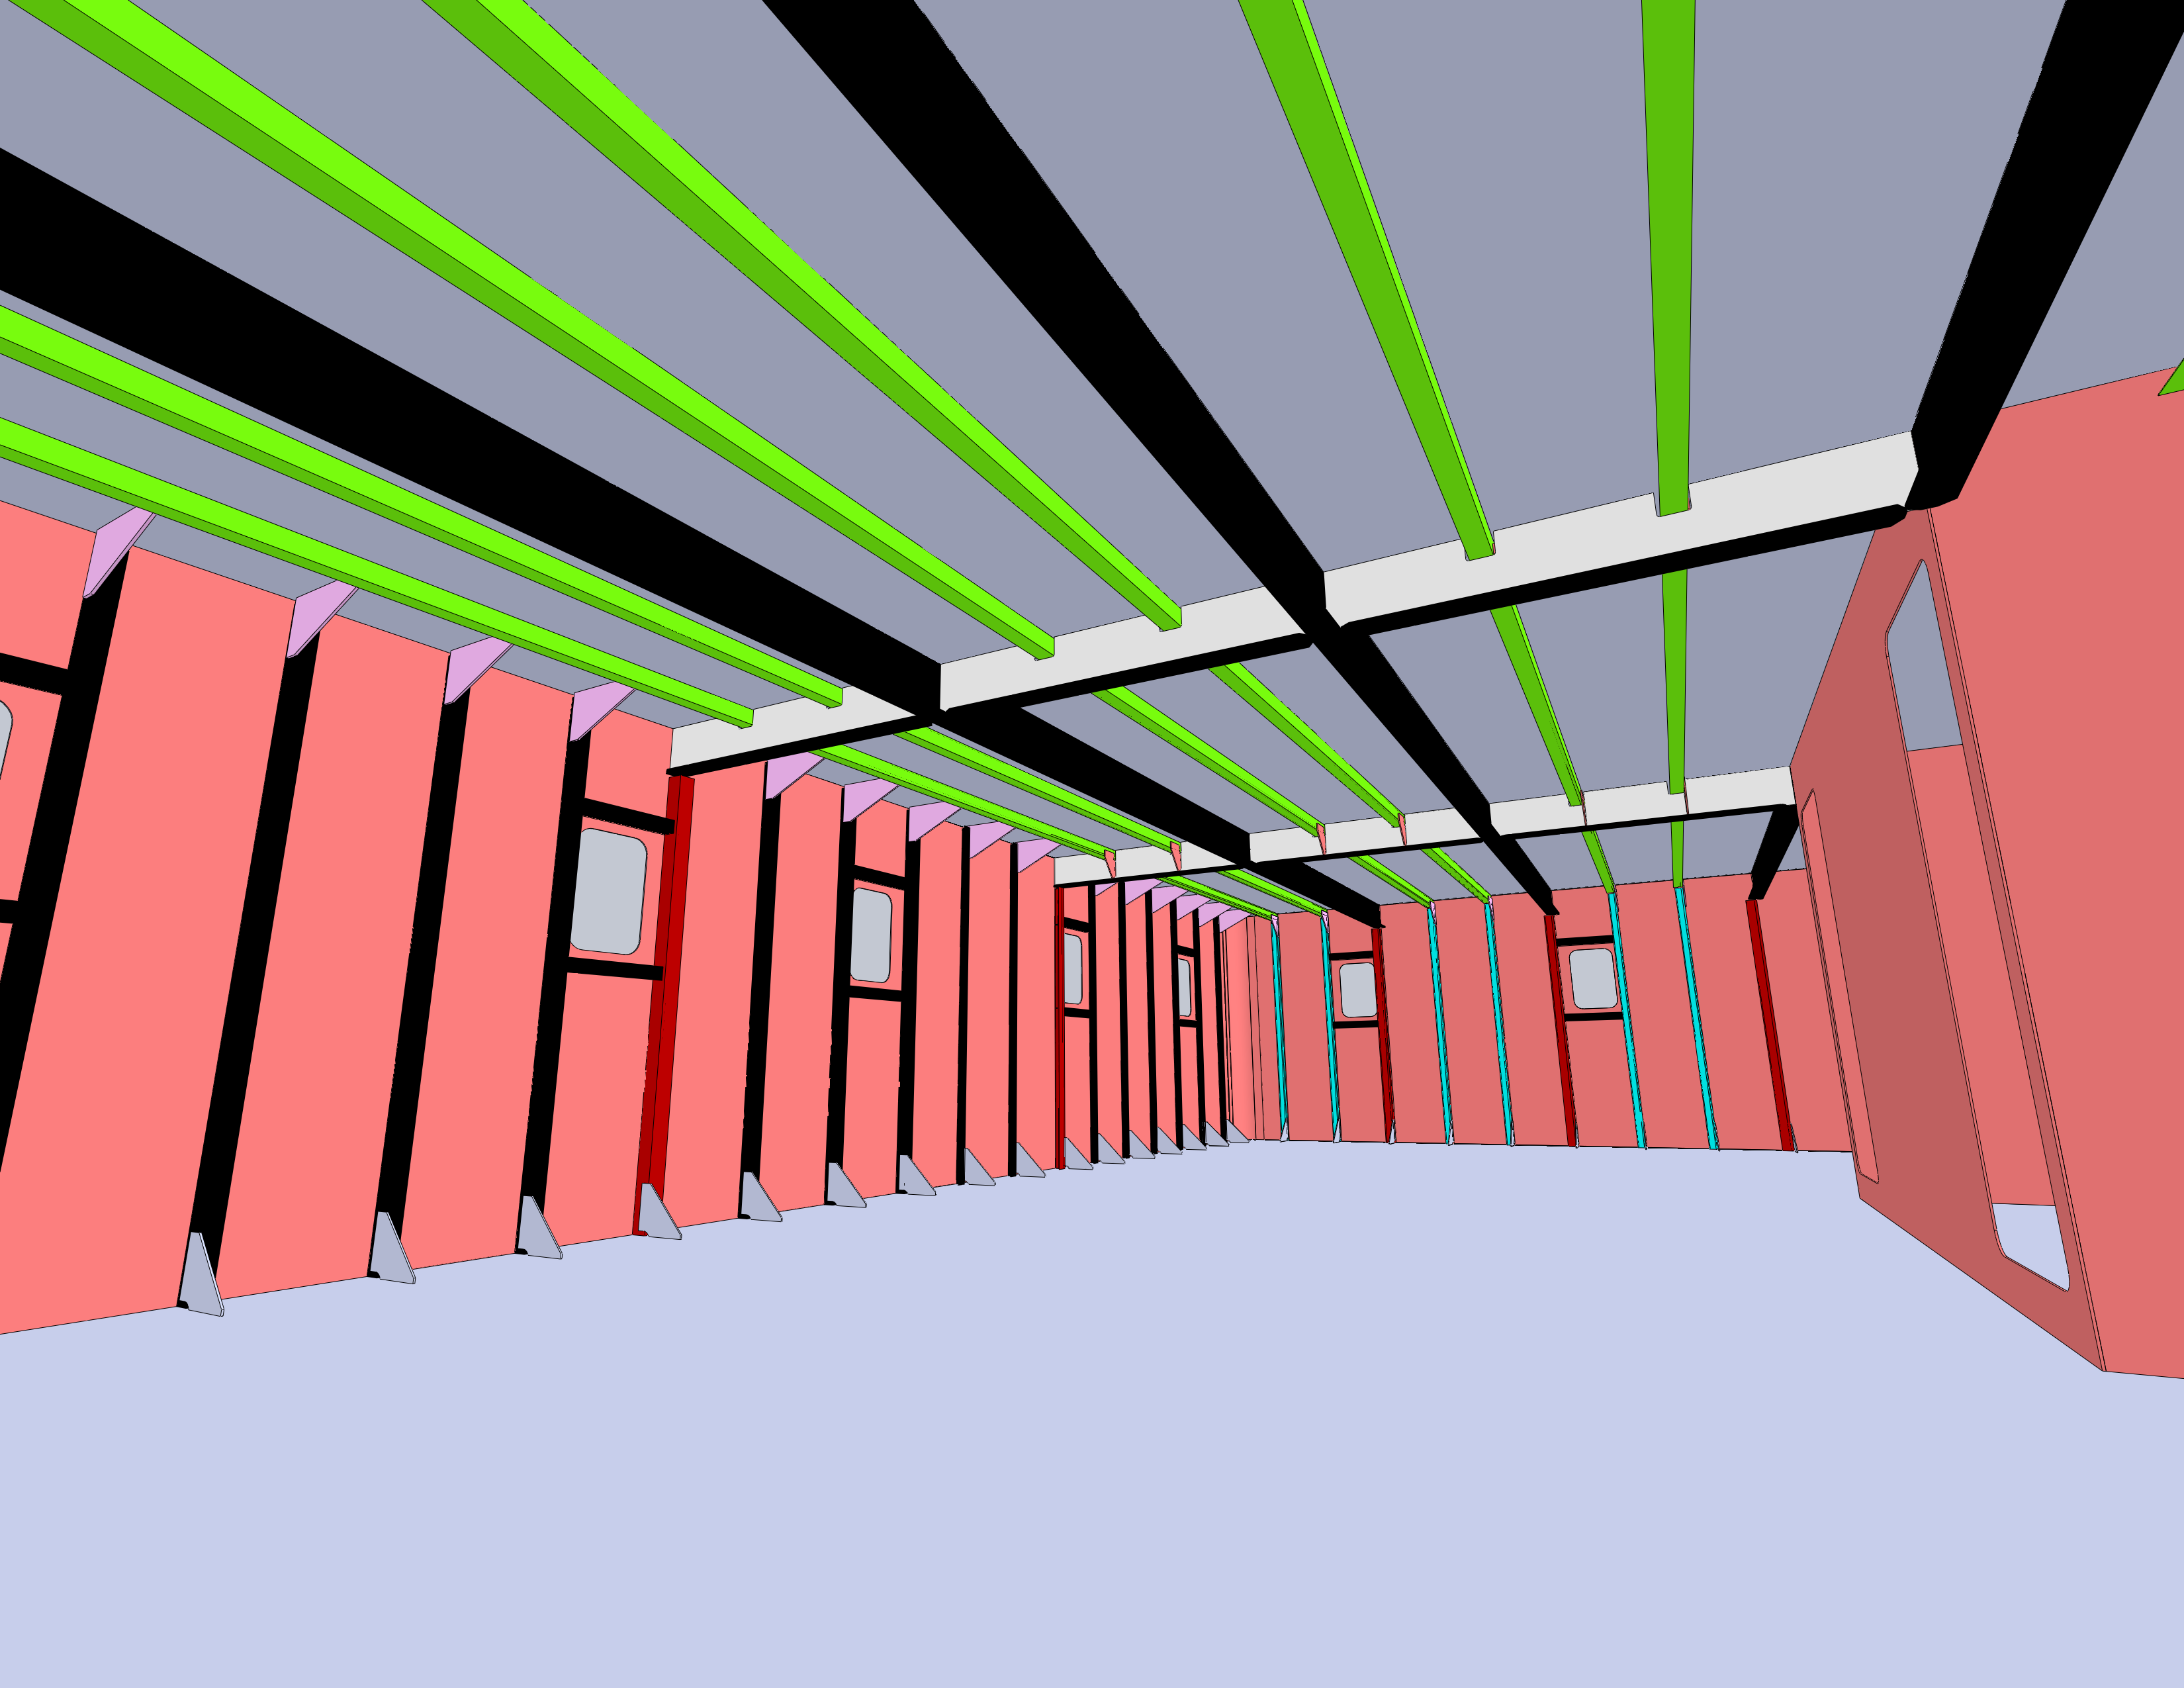
\includegraphics[width=\textwidth]{localization-system-evaluation/testing-environments/guardian-environment-inside}
	\end{subfigure}
	\caption{Guardian testing environment}
	\label{fig:localization-system-evaluation_guardian-tests-environment}
\end{figure}

\begin{figure}[H]
	\centering
	\begin{subfigure}[ht]{0.4\textwidth}
		\centering
		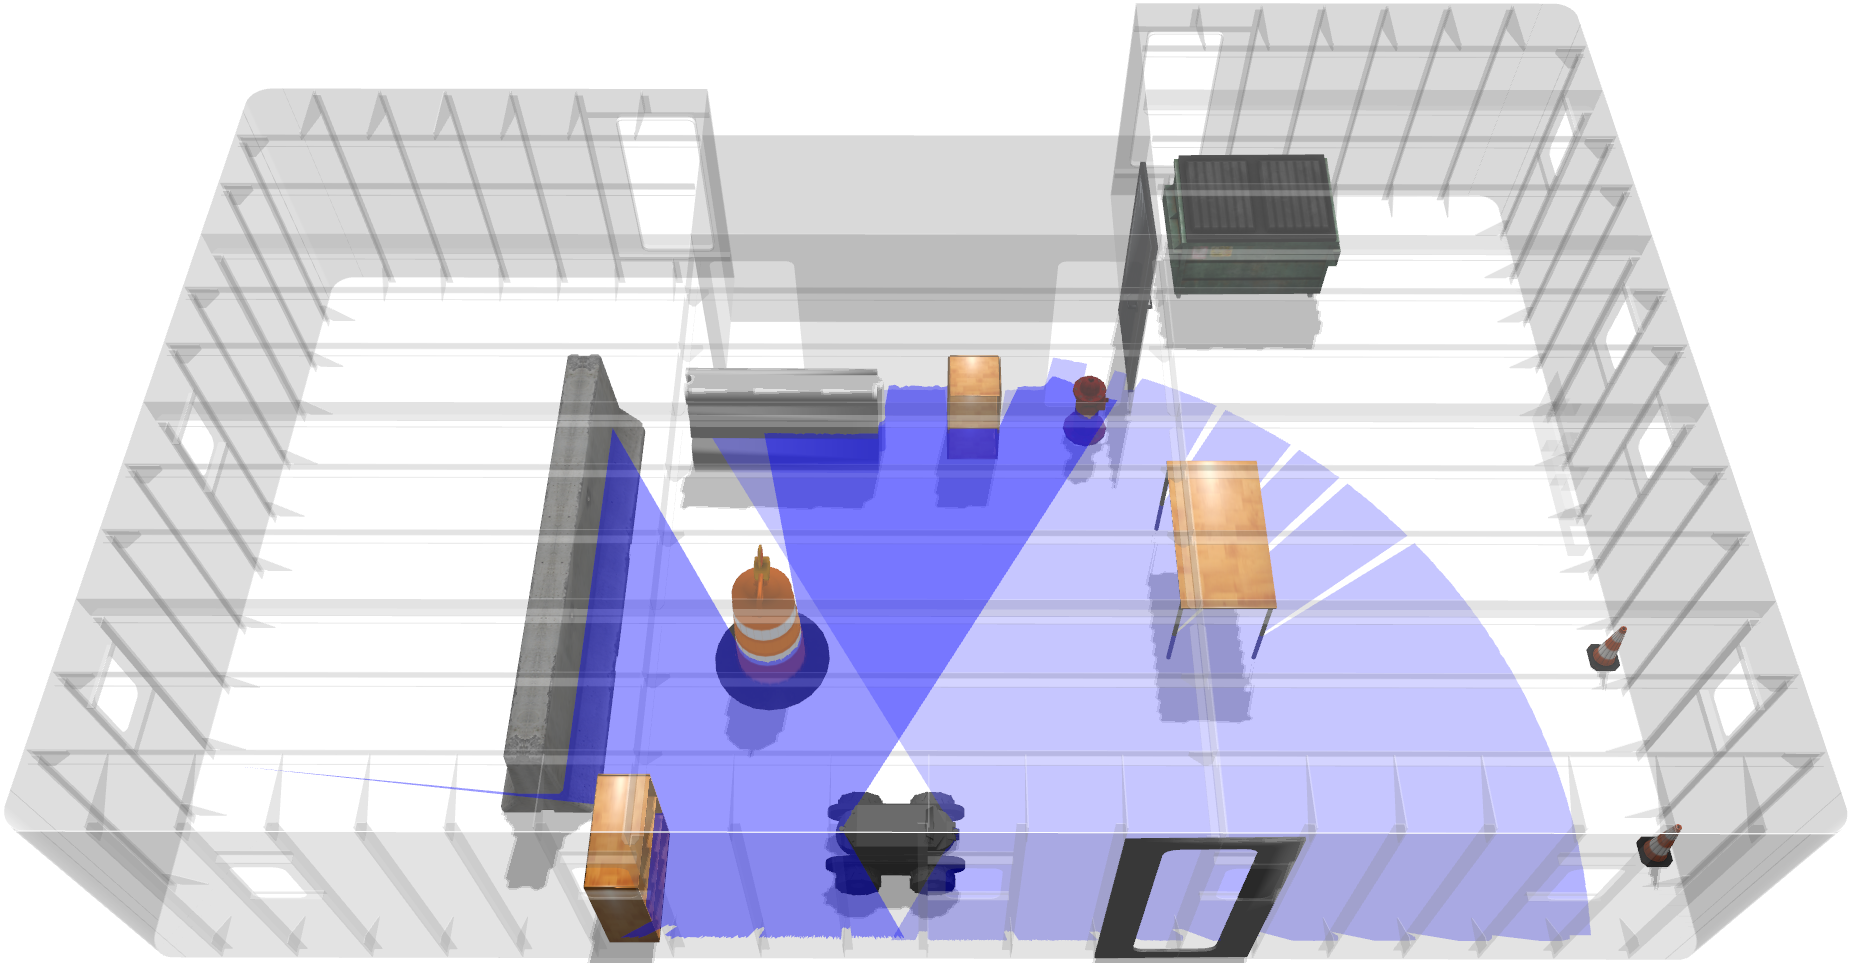
\includegraphics[width=\textwidth]{localization-system-evaluation/testing-environments/guardian-environment-cluttered}
	\end{subfigure}
	\begin{subfigure}[ht]{0.4\textwidth}
		\centering
		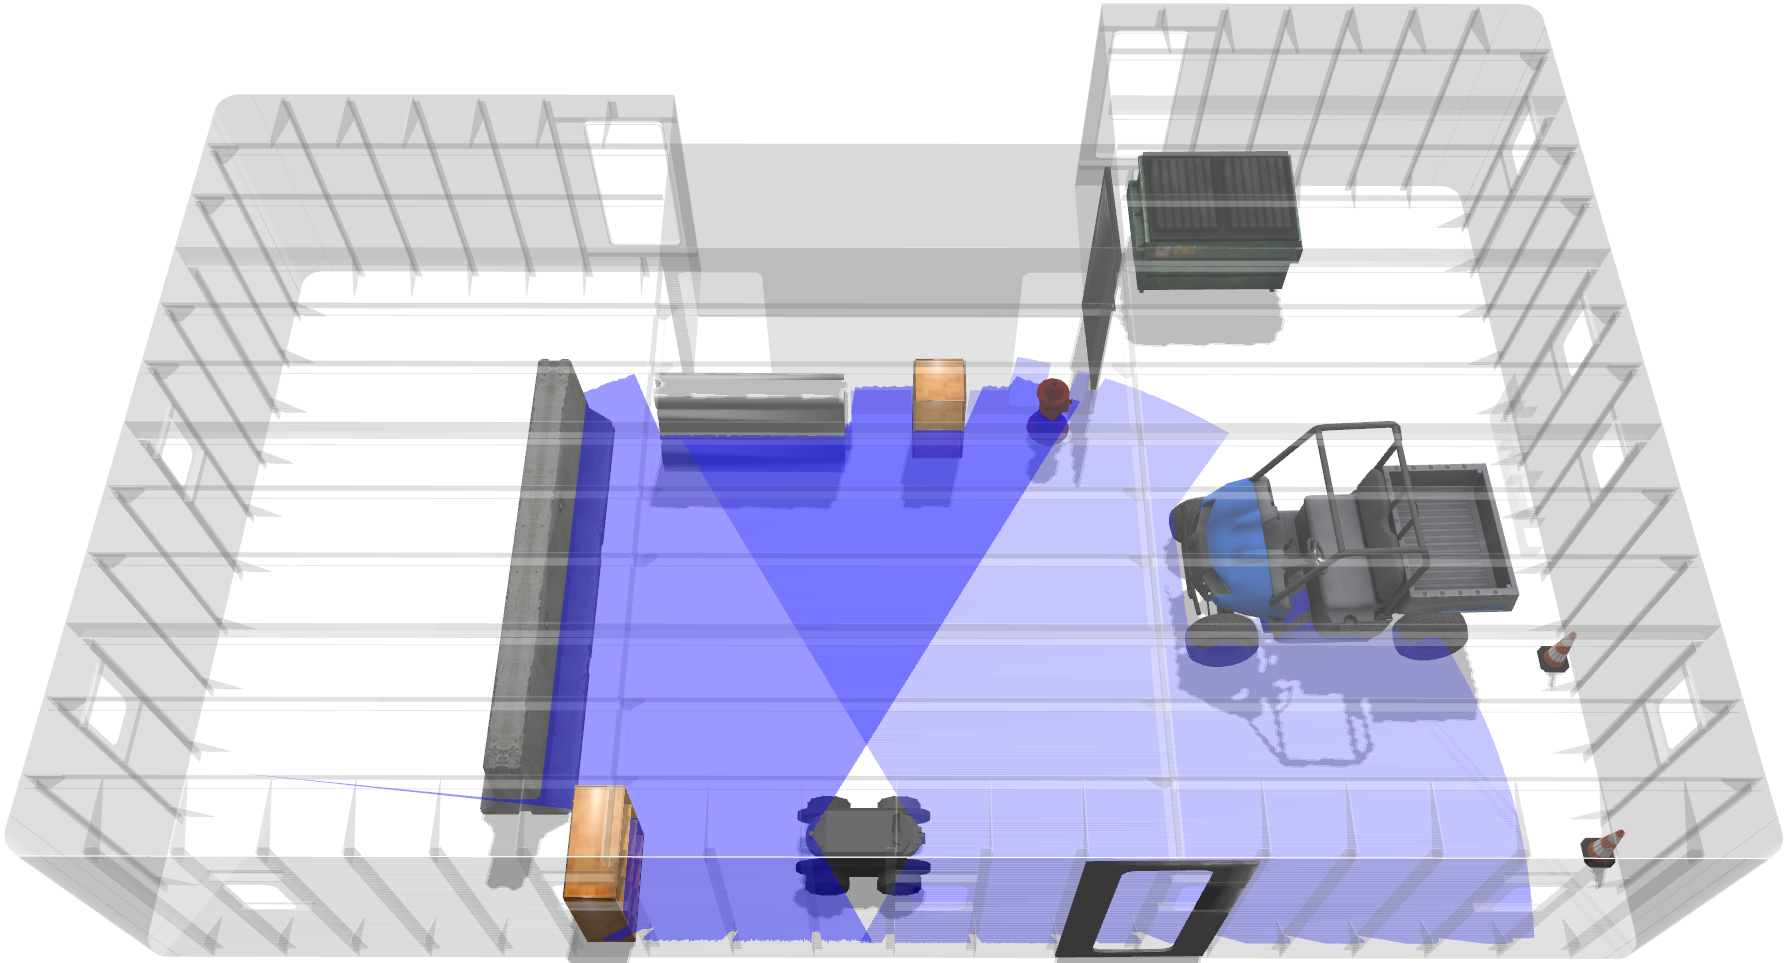
\includegraphics[width=\textwidth]{localization-system-evaluation/testing-environments/guardian-environment-cluttered-dynamic}
	\end{subfigure}
	\caption{Guardian cluttered (top) and dynamic (bottom) testing environments}
	\label{fig:localization-system-evaluation_guardian-tests-environment-cluttered}
\end{figure}



\subsubsection{Pioneer in industrial hall}

One of the datasets presented in \cite{Sturm2012} is a industrial hall consisting of a large room with several tables and objects spread around. Four tests were performed with a Pioneer 3-DX in this environment. The first was a 360º path with few camera supports in the middle of the room, while the remaining 3 were done with a lot of large objects, that significantly reduced the field of view of the robot laser (as can be seen in \Cref{fig:localization-system-evaluation_industrial-hall}).

\begin{figure}[ht]
	\centering
	\begin{subfigure}[ht]{0.37\textwidth}
		\centering
		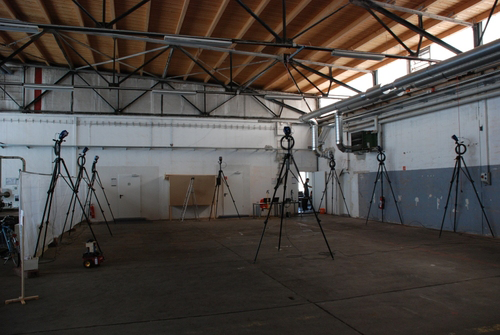
\includegraphics[width=0.95\textwidth]{localization-system-evaluation/testing-environments/industrial-hall-1}
	\end{subfigure}
	\begin{subfigure}[ht]{0.44\textwidth}
		\centering
		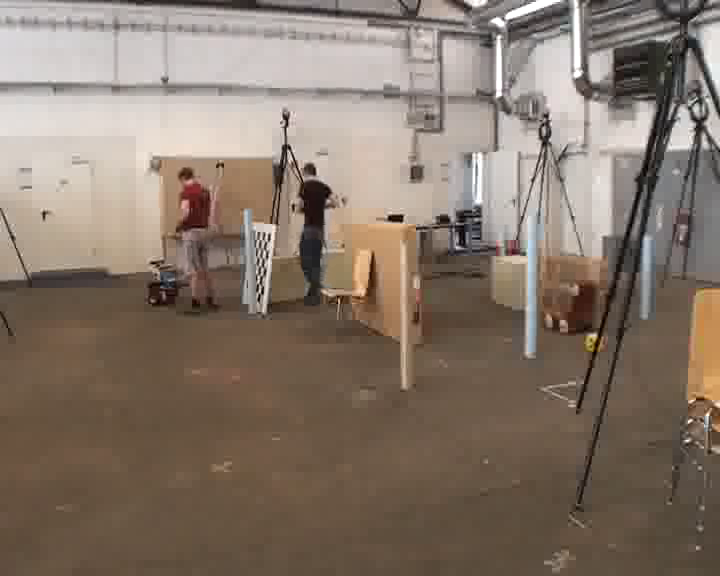
\includegraphics[width=0.8\textwidth]{localization-system-evaluation/testing-environments/industrial-hall-2}
	\end{subfigure}
	\caption{Industrial hall with (top) and without (bottom) objects in the center \cite{Sturm2012}}
	\label{fig:localization-system-evaluation_industrial-hall}
\end{figure}



\subsubsection{Kinect in flying arena}

The flying arena dataset introduced in \cite{Pomerleau2011} and shown in \Cref{fig:localization-system-evaluation_flying-arena} is a large room in which several objects were added to test 6 \gls{dof} pose tracking. In these tests the Kinect was moved by the operator in three different paths. The first was a smooth fly movement over the testing scene, while the other two aimed to test paths with mainly translations and rotations. This environment had a ground truth provided by Vicon cameras\footnote{\url{http://www.vicon.com/}} and according to the authors of the dataset \cite{Pomerleau2011} it had sub-centimeter accuracy.

\begin{figure}[H]
	\centering
	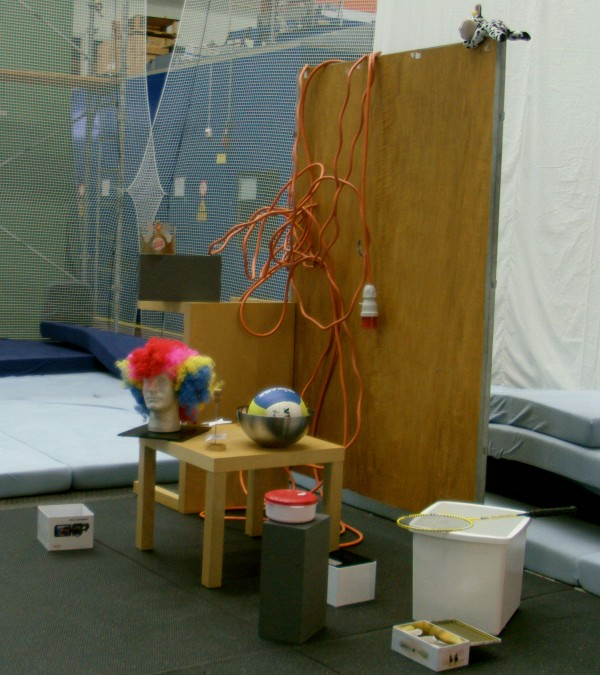
\includegraphics[width=0.35\textwidth]{localization-system-evaluation/testing-environments/kinect-flying-arena}
	\caption{Flying arena environment \cite{Pomerleau2011}}
	\label{fig:localization-system-evaluation_flying-arena}
\end{figure}
